\section{KnoBAB Architecture}\label{sec:karch}
The methodology behind its design systematically follows the major architectural components of a relational database, with the only bespoke characteristics of tailoring such solution to the specific problem that we intend to solve (\S\ref{ssec:xltlf}), that is, computing either the MSP for each log trace,  or the \textsc{Support} associated to each model clause, or computing the traces satisfying all of the model clauses (\textit{conjunctive query}).

\begin{figure}[!t]
	\centering
	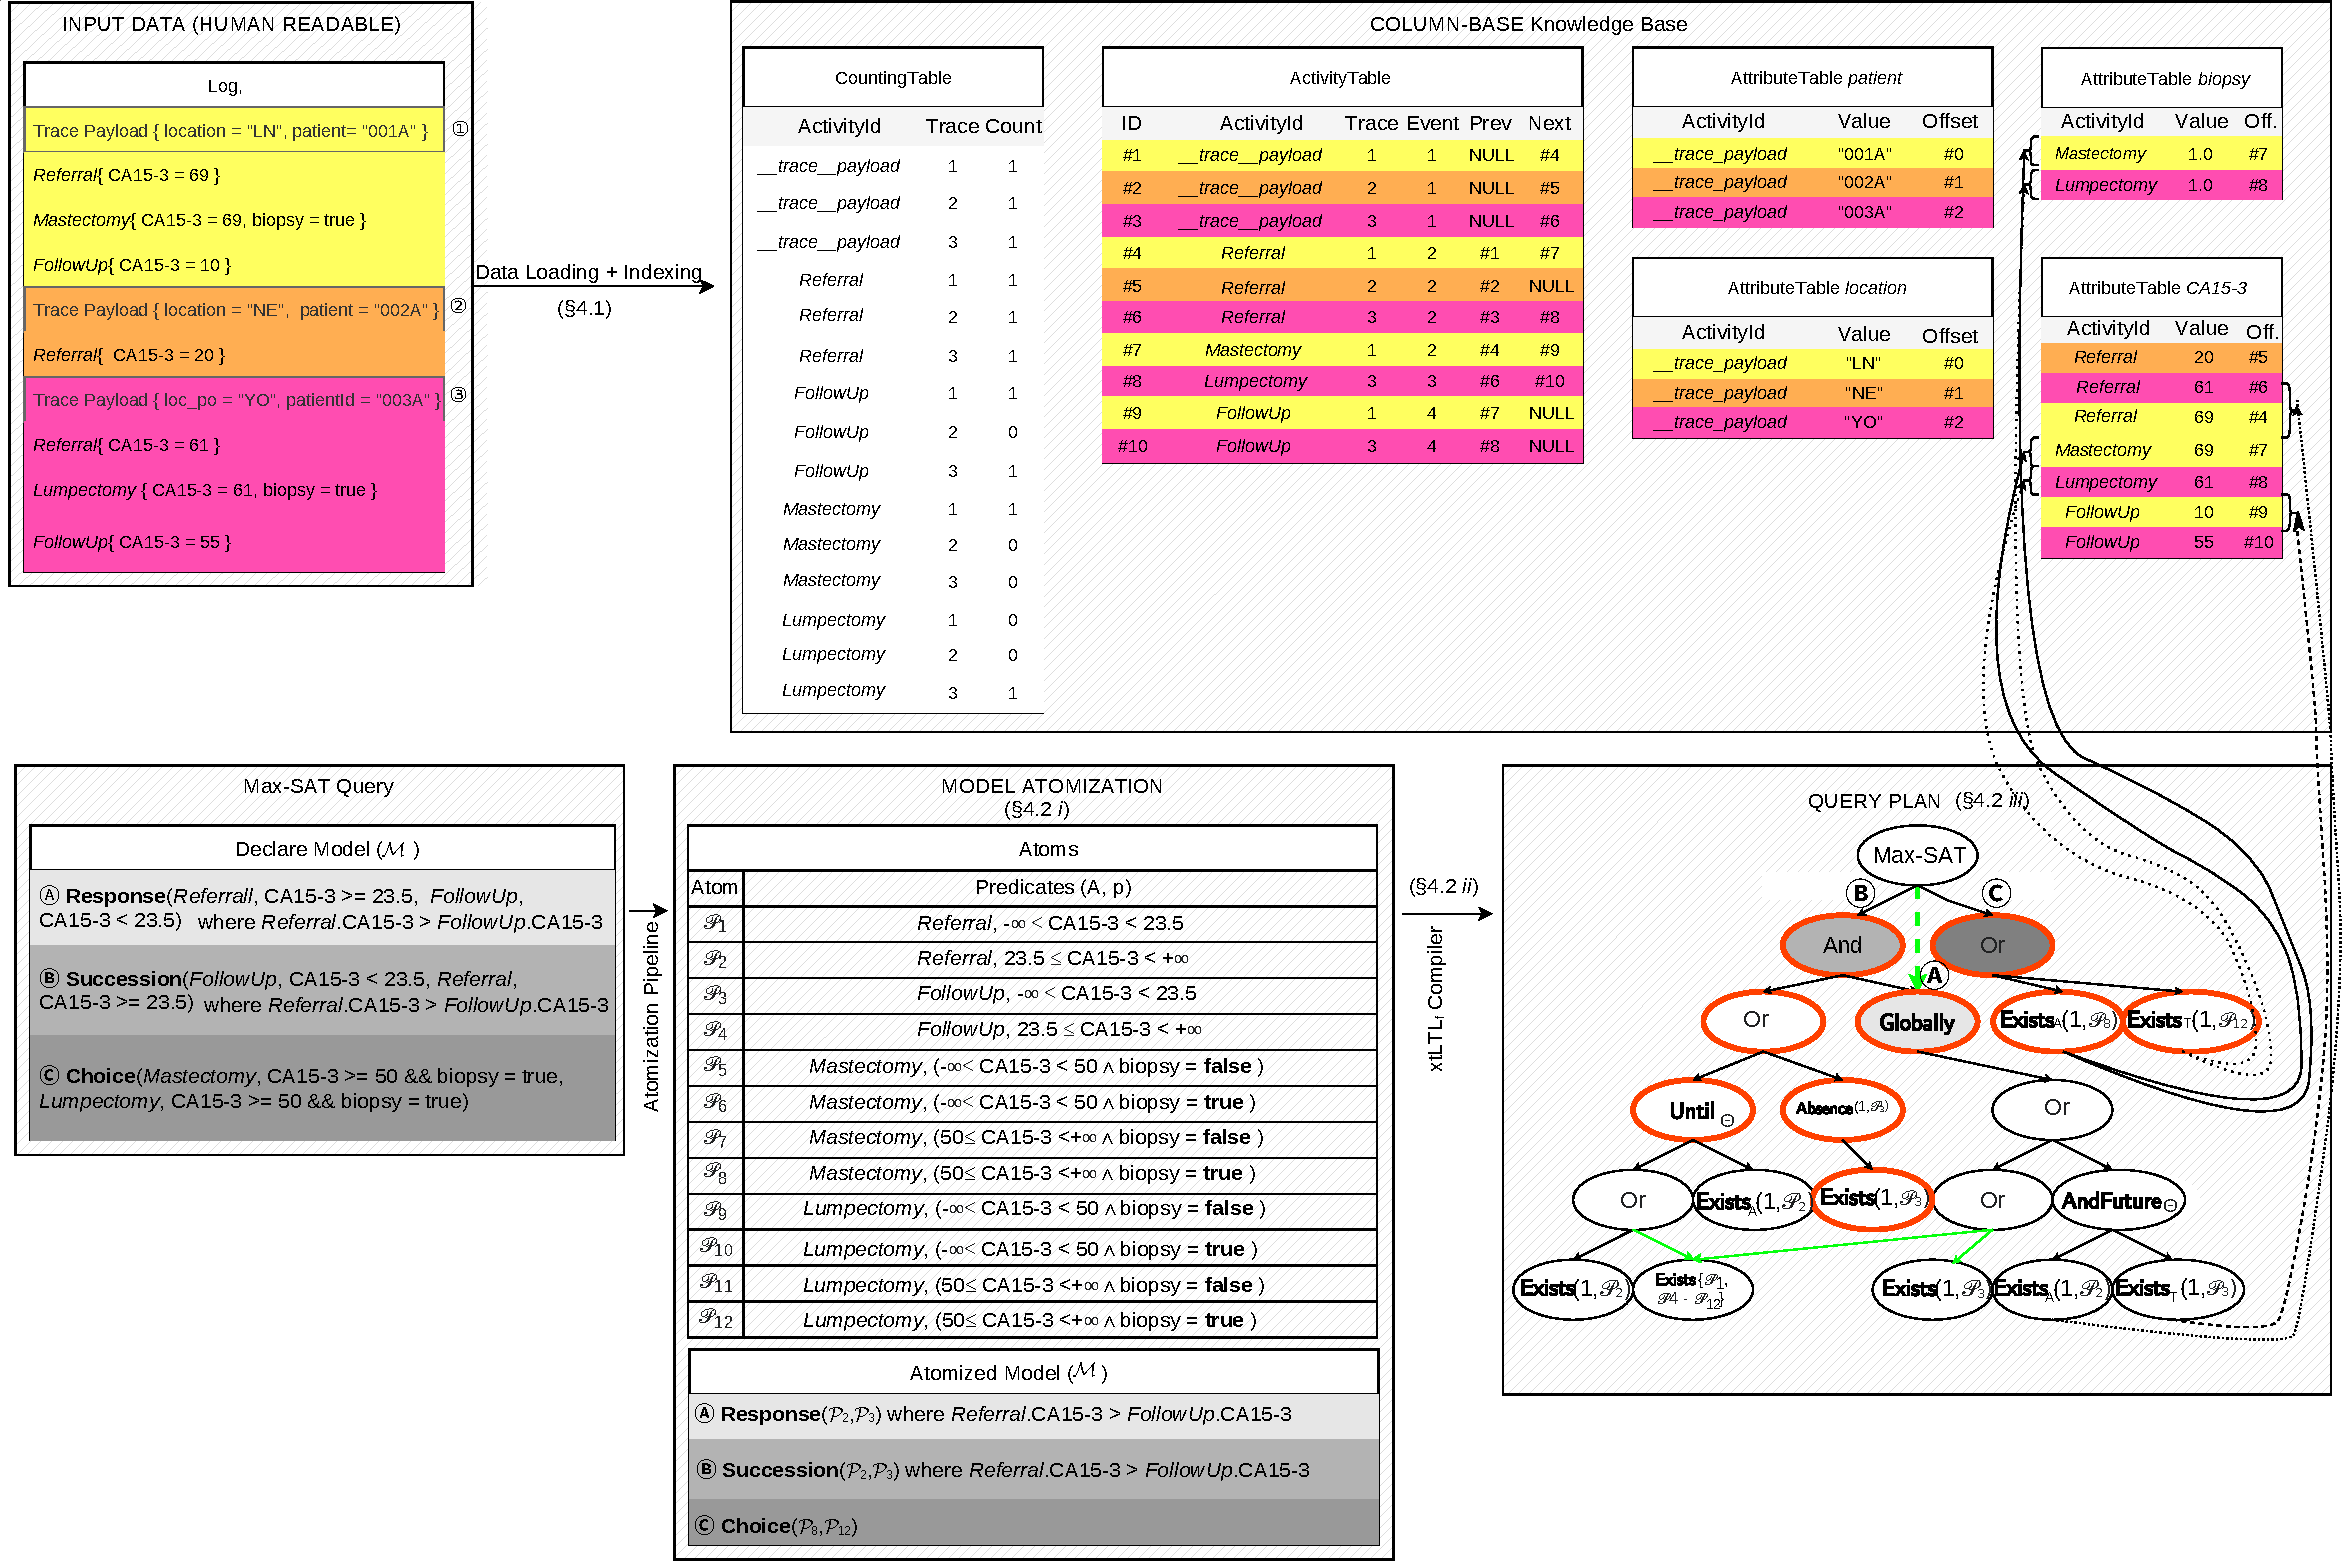
\includegraphics[width=.7\textwidth]{images/knobab_pipeline.pdf}
	\caption{KnoBAB vs SQLMiner Performance for Varying Model Size.}\label{fig:vsSQL}
\end{figure}

